\chapter{Conclusion}
\label{ch:conclusion}

\section{Summary of Findings}

We set out to learn which design choices govern which aspects of reliability when a frozen lightweight
CNN is adapted for few-shot classification with a small trainable adapter. \Cref{tab:conclusion}
summarises the answers.

\begin{table}[H]
\centering
\caption{What this thesis found: no single design choice optimises every reliability aspect.}
\label{tab:conclusion}
\begin{tabularx}{\textwidth}{@{}l>{\raggedright\arraybackslash}p{3.6cm}X@{}}
\toprule
Aspect & Main factor & Evidence \\
\midrule
Accuracy & shot count, then adapter architecture & 76\% of accuracy variance from shots; bottleneck wins 16/16 grid pairs and 8/8 at matched budget \\
Calibration & head, then backbone & 83\% of ECE variance from the head; at matched budget, backbone rule 3/4 cells, budget rule 0/4 \\
OOD detection & scoring rule & 42.7\% of far-OOD variance from the score vs.\ 0.17\% from the training objective \\
Calibration repair & two-parameter refit & ECE improved in 60/60 evidential models, still worse than softmax in 60/60 \\
\bottomrule
\end{tabularx}
\end{table}

A 31.7K-parameter parallel bottleneck adapter beats full fine-tuning of an 11.18M-parameter ResNet-18 at
5-shot and comes within 2.6 points of it at 1-shot. Accuracy is driven mainly by the number
of shots and then by the adapter's architecture, and the head barely affects it. Calibration is driven by
the head: the evidential head is worse calibrated than softmax in all 20 matched pairs. The evidential head
looked like a better OOD detector, but separating training objective from scoring rule shows that this
advantage belongs to the score; the parameter-free energy score is the strongest score in most settings and
works almost equally well on evidential-trained logits. When the two adapters are given the same parameter
budget, the bottleneck still wins on accuracy and near-OOD detection, while the calibration gap stays with
the backbone. Finally, refitting the evidential head's two evidence parameters after training improves its
calibration in every model but does not make it as well calibrated as softmax, and it lowers OOD AUROC by more
than 0.005 in a fifth of the comparisons.

\begin{figure}[H]
\centering
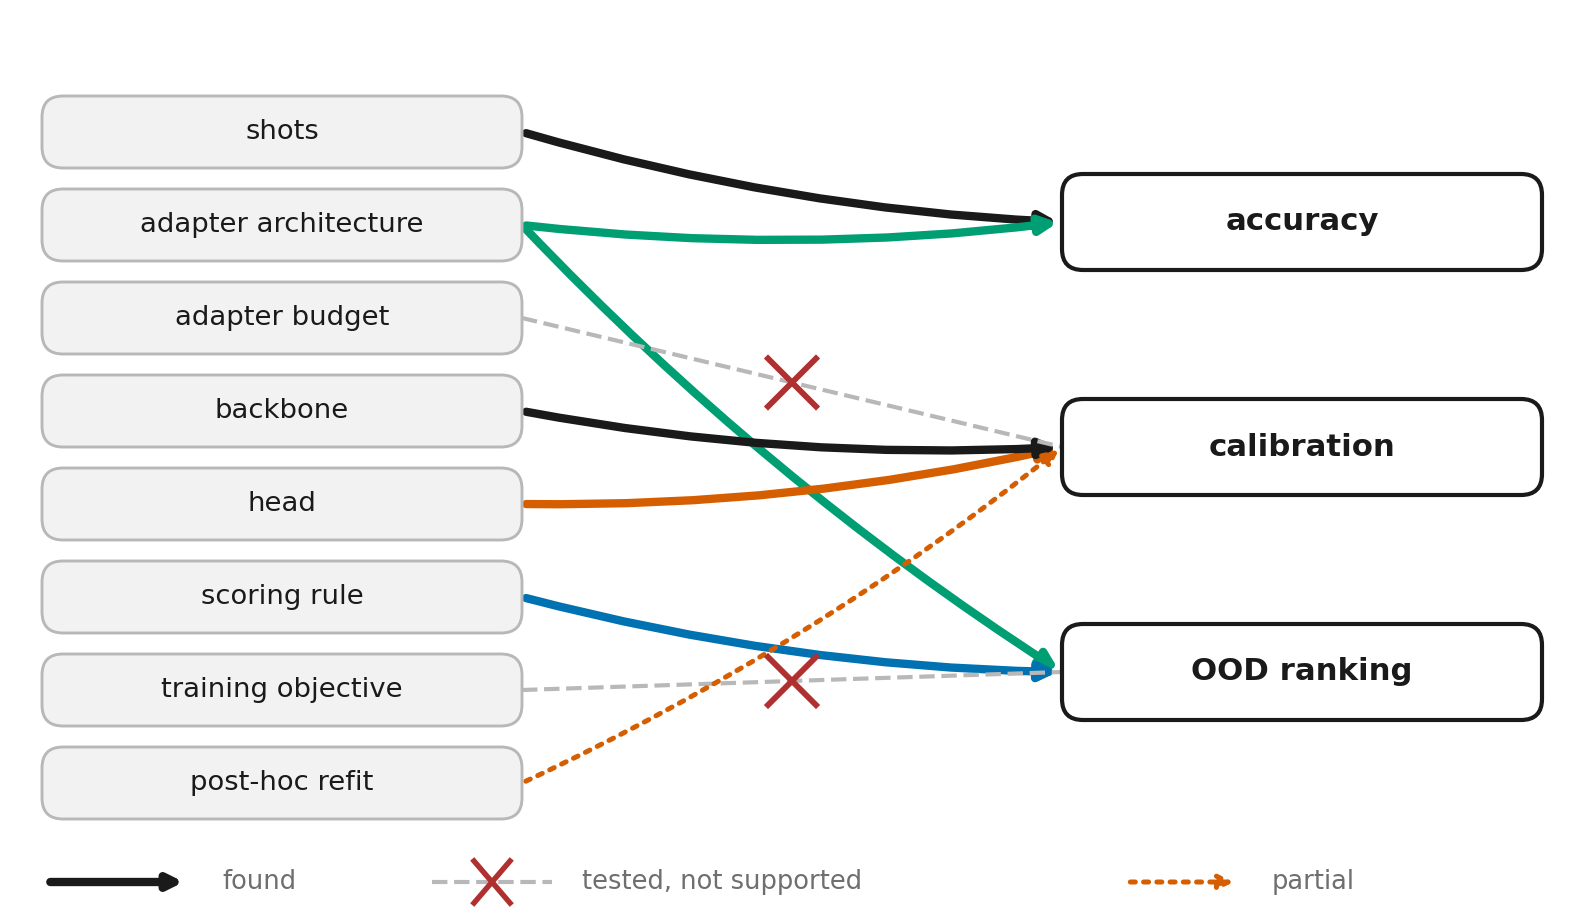
\includegraphics[width=0.9\textwidth]{F16_findings_graph.png}
\caption{Each design factor against each reliability outcome: links that were found, links that were tested
and not supported, and partial links.}
\label{fig:findings}
\end{figure}

The main contribution is therefore not a better model but a controlled decomposition of which design
choices govern which aspects of reliability in this few-shot PEFT setting.

\section{Contributions}

\begin{itemize}
\item A controlled comparison of adapters on frozen lightweight CNNs that reports accuracy, calibration and
OOD detection for the same 120 models.
\item A variance decomposition showing that accuracy and calibration are controlled by largely different
factors (RQ1).
\item A crossing of training objectives with scoring rules showing that OOD detection is decided by the
score, including the finding that energy transfers almost unchanged to evidential-trained models (RQ2).
\item A pre-registered matched-budget design that separates adapter architecture from parameter budget and
shows that calibration follows the backbone, not the budget (RQ3).
\item A measured two-parameter post-hoc refit of the evidential head, reporting both its benefit and its
cost in OOD ranking (RQ4).
\end{itemize}

\section{Limitations}

The limitations are discussed in \cref{sec:limits}. The most important are the ImageNet pretraining
overlap with MiniImageNet's test classes, the use of only two backbones, a single shared training recipe,
and three seeds that vary only the adapter's initialisation.

\section{Future Work}

\begin{itemize}
\item \textbf{More backbones.} The most important next step is to add backbones that vary depth, width,
normalisation and block type one at a time, to find which backbone property decides which adapter is better
calibrated.
\item \textbf{Separating the parts of ``architecture''.} Variants of the two adapters that differ in only one
respect (non-linearity, number of insertion points, or branch versus weight update) would show what makes
the bottleneck more accurate.
\item \textbf{A transformer arm.} Running a small ViT under exactly our protocol would replace the
literature comparison of \cref{sec:sota} with a direct measurement.
\item \textbf{Pretraining control.} A backbone pretrained without the MiniImageNet test classes would measure
the size of the pretraining overlap instead of only noting it.
\end{itemize}

\section{Concluding Remarks}

We began by asking whether an evidential uncertainty mechanism makes a parameter-efficient, lightweight CNN
more reliable in the few-shot regime. The answer turned out to be more specific than yes or no. The
evidential head ranks unfamiliar inputs better than softmax probabilities do, but a free score on ordinary
softmax logits does as well or better in most settings, and the evidential head pays for it with worse calibration that a
small post-hoc refit only partly repairs. Which adapter to use, which backbone to use and how to score
uncertainty each turned out to matter for a different part of reliability, and only a controlled design
could tell them apart.
